We will now use the above derived equation in a homogeneous magnetic field, assuming cold ions and constant electron temperature in a cylindrical geometry.

The resulting model will from here be referred to as the CELMA model, an abbrevation of \textbf{C}onsistent \textbf{E}quations in a \textbf{L}inear \textbf{MA}chine%
\footnote{
    This should not be confused with PELMA, \textbf{P}erfect \textbf{E}quations in a \textbf{L}inear \textbf{MA}chine.
    As we have seen, there is an inconsistent approximation to use a constant temperature whilst $\frac{u^c}{c^c_s}\simeq\sqrt{\e}$, but this approximation is consitently implemented.
}%
.

We will end up with a coupled set of four PDEs, which solves the density, the sum of the parallel momentum densities, the current and the modified vorticity in time (plus a boundary equation which gives the potential at the given timestep).
In other words, we have managed to considerably reduce the original system containing of eigth coupled PDEs.
The final set of equation is found in \cref{eq:celma_vortD,eq:celma_dens,eq:celma_mom_dens,eq:celma_j_par,eq:celma_vortD_evolution}.

The aim is to model something similar to what is observed in linear plasma devices.
Several types of linear machines exsists, all with different purposes.
For example has the Q-machines have been used for the study quiescent alkali plasmas \cite{Nielsen1996} and machines like Magnum-PSI \cite{Rapp2010} are mainly used for the study plasma-wall interactions.
Here, we would restrict our attention to mainly helicon type plasmas, where a helicon wave are responsible for the plasma creation \cite{Boswell1984,Shamrai1996}.
No momentum is added to the plasma in this creation process.
The plasma creation process will in this thesis therefore just be approximated by the source variable $S_n$, which we keep constant in time.

Helicon devices operationable during the writing of this thesis includes VINETA \cite{Schroder2005}%
\footnote{Now VINETA II \cite{Bohlin2014}, mainly used for magnetic reconnection studies.}%
%
(depicted in \cref{fig:VINETA}), PANTA (previously LMD-U) \cite{Oldenburger2012} and CSDX \cite{Tynan2004a}.
%
\begin{figure}[htb]
    \centering
    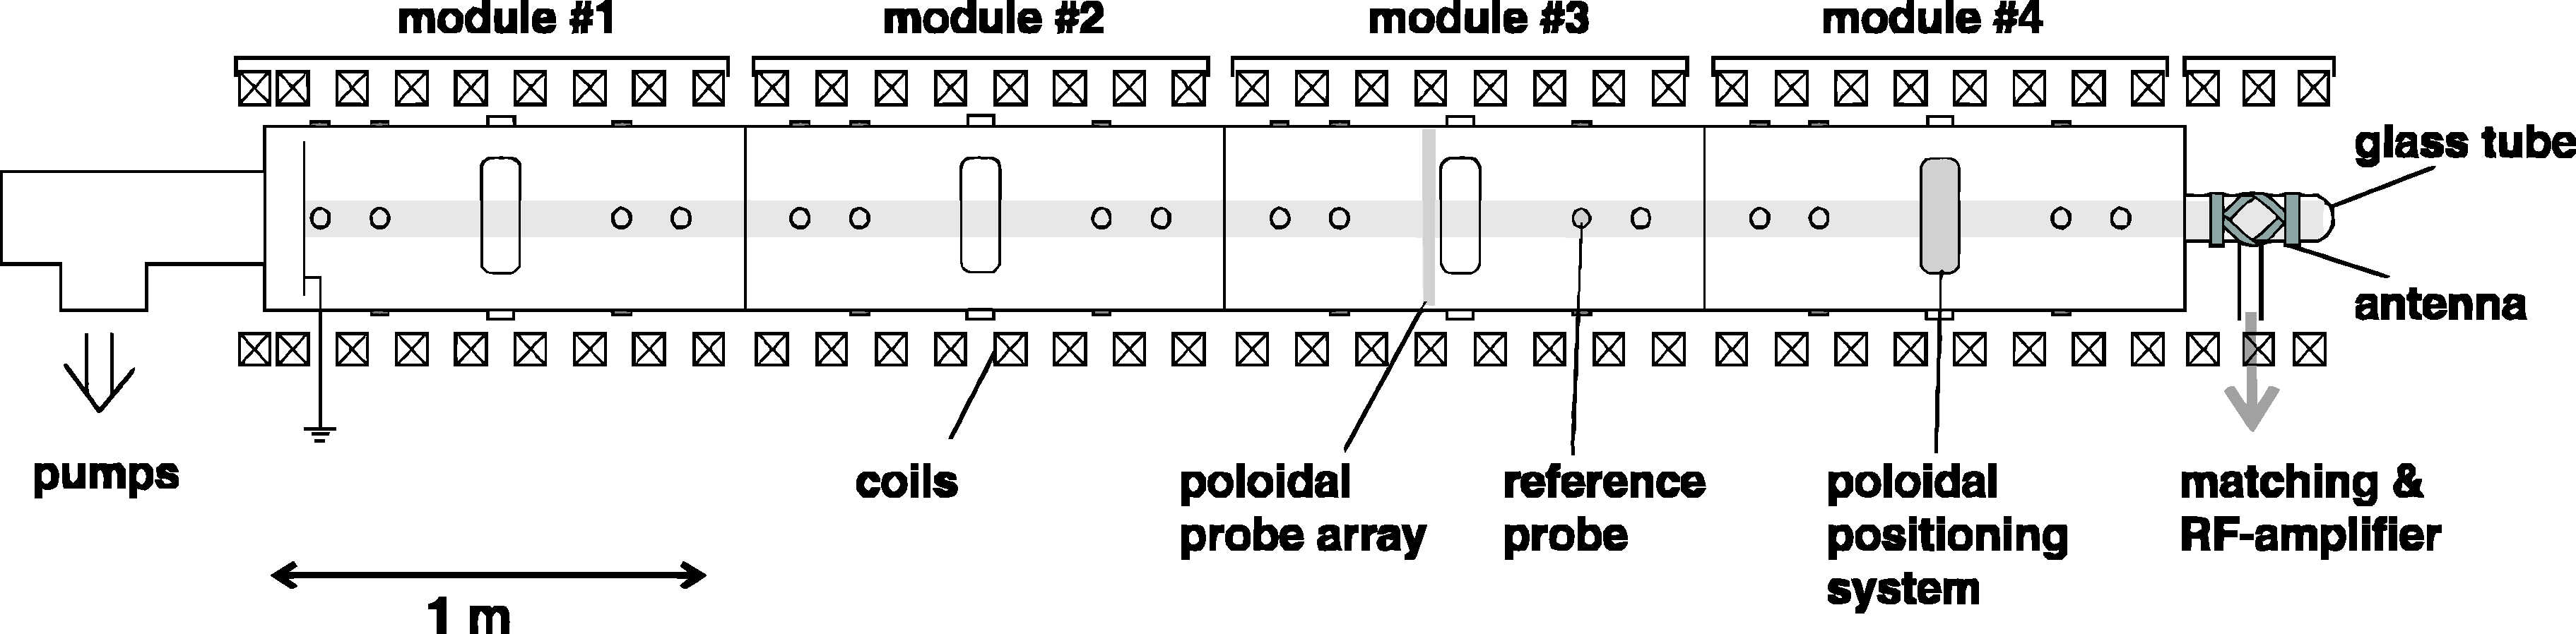
\includegraphics[width=1.0\textwidth]{fig/VINETA}
    \caption{Sketch of VINETA (from \cite{Schroder2005}).}
    \label{fig:VINETA}
\end{figure}
%
Although we restrict our scope to helicon devices, machines like the LAPD \cite{Gekelman1991,Gekelman2016} are also possible to model with CELMA by proper adjusting of $S_n$.

\section{The density equation}
%
We will now rewrite the electron density equation (\cref{eq:dens_evol_gen}) using that we are in a straight magnetic field (so that $B=\text{const}$ and $\mathcal{C}(f)=0$) using the assumptions that the electron temperature is constant and the ion temperature is negligible.
This yields
%
\begin{align*}
    \d_t^E n
    &=
    - n\mathcal{C}(\phi)
    + \frac{1}{e}\mathcal{C}(\phi)
    +\frac{1}{\mu}\frac{m_i\nu_{ei}}{e^2}
    \div\L( \frac{\grad_\perp \L(p_e + p_i\R)}{B^2} \R)
    - \div\L(n \ve{u}_{e,\|}\R)
    + S_{n}
    \note{$p_i=0$\\$B=\text{const}$}
    \\
%
    &=
  \frac{1}{\mu}
  \frac{m_iT_e\nu_{ei}}{B^2e^2}
   \grad_\perp^2 n
   - \div\L(n \ve{b}u_{e,\|}\R)
   + S_n
   \note{$\partial_i \ve{b} = 0$}
    \\
%
    &=
  \frac{1}{\mu}
  \frac{m_iT_e\nu_{ei}}{B^2e^2}
   \grad_\perp^2 n
   - \ve{b}\cdot\grad \L(n u_{e,\|}\R)
   + S_n
    \\
%
    &=
  \frac{1}{\mu}
  \frac{m_iT_e\nu_{ei}}{B^2e^2}
   \grad_\perp^2 n
   - \partial_\| \L(n u_{e,\|}\R)
   + S_n.
\end{align*}
%
Using that
$\rho_s=\frac{c_s}{\om_{ci}}=\sqrt{\frac{T_e}{m_i}}\frac{m_i}{eB}
       =\sqrt{\frac{T_em_i}{e^2B^2}}$
we find that
%
\begin{align}
    \d_t^E n
    &=
  \frac{\rho_s^2\nu_{ei}}{\mu}
   \grad_\perp^2 n
   - \partial_\|\L(n u_{e,\|} \R)
   + S_n.
    \label{eq:non_norm_dens}
\end{align}

\section{The vorticity equation}
%
We will in the section derive an equation which can be used to find the evolution of the vorticity.
Strictly speaking, the vorticity $\Om$ of a fluid field is defined as $\curl \ve{u}$.
Thus, $\Om$ tells us something about the rotation of the fluid field.
In this thesis, a slightly different definition will be used:
%
\begin{align*}
    \frac{\grad^2_\perp \phi}{B} \defined \Om.
\end{align*}
%
Note that this is only the parallel part of the rotation of the advective vorticity:
%
\begin{align*}
    \L(\curl \ve{u}_E\R)\cdot\ve{b}
    &=
    \L(-\curl \frac{\grad \phi \times \ve{b}}{B}\R)\cdot\ve{b}
    \note{$\grad \frac{1}{B}\simeq 0$}
    \\
%
    &=
    \frac{1}{B}\L(\curl \ve{b} \times \grad \phi \R)\cdot\ve{b}
    \note{$\curl (\ve{A}\times\ve{B}) = \ve{A}(\div\ve{B}) - \ve{B}(\div\ve{A})
                        + (\ve{B}\cdot\grad)\ve{A} - (\ve{A}\cdot\grad)\ve{B}$}
    \\
%
    &=
    \frac{1}{B}\L(   \ve{b}\L[\div\grad\phi\R]
                   - \grad\phi\L[\div\ve{b}\R]
                   + \L[\grad\phi\cdot\grad\R]\ve{b}
                   - \L[\ve{b}\cdot\grad\R]\grad\phi
               \R)\cdot\ve{b}
    \\
%
    &=
    \frac{1}{B}\L(   \ve{b}\L[\div\grad\phi\R]
                   - \L[\ve{b}\cdot\grad\R]\grad\phi
               \R)\cdot\ve{b}
    \note{$\div \ve{b} \simeq 0$ and $\grad \ve{b} \simeq 0$}
    \\
%
    &=
    \frac{1}{B}\L( \ve{b} \cdot \ve{b}\L[\div\grad\phi\R]
                   - \ve{b} \cdot \L[\ve{b}\cdot\grad\R]\grad\phi \R)
    \\
%
    &=
    \frac{1}{B}\L( \grad^2\phi
                   - \ve{b} \cdot \L[\grad\ve{b}\cdot\R]\grad\phi \R)
               \\
%
    &=
    \frac{1}{B}\L( \grad^2\phi
                   - \L[ \ve{b} \cdot \grad \R]\ve{b}\cdot\grad\phi \R)
               \\
%
    &=
    \frac{1}{B}\L( \grad^2\phi
                   - \div \L[ \ve{b} \ve{b}\cdot\grad\phi \R] \R)
               \\
%
    &=
    \frac{1}{B}\L(\grad_\perp^2\phi \R),
\end{align*}
%
where we in the last line have used that
$
\grad^2_\perp = \grad^2 - \grad_\|^2 = \grad^2 -
                   \div \L[ \ve{b} \ve{b}\cdot\grad \R]
                   $.
%
Such a term would pop up (amongst other terms) if we took the divergence of the polarization drift defined in \cref{eq:first_order}.
However, we will derive the voriticity equation from the conservation of charge (see \cref{eq:current_drifts}), where we already have a term on the form $\div(n\ve{u}_{i,p})$.
As such, it makes sense to define the density modified voriticity $\Om^D$ (or simply just "the modified voriticity") as
%
\begin{align}
    \Om^D \defined
    \div \L(n \frac{\grad_\perp \phi}{B} \R).
    \label{eq:omDDef}
\end{align}
%
In the end, we will evolve $\Om^D$ in time unless we use the Boussinesq approximation (see \cref{chap:boussinesq}).
When the Boussinesq approximation is invoked, we will instead evolve $\Om$.
In order to derive two equations, we will start by investigating the left hand side of \cref{eq:full_vort_eq} term by term.

\subsection{The diamagnetic contribution}
%
\begin{align*}
    \frac{1}{e}\L[\mathcal{C}(p_e+p_i)\R].
\end{align*}
%
disappears as $\mathcal{C}(f)$ vanishes for a straight magnetic field.

\subsection{The neutral contribution}
%
The two next terms, which originate from the Pedersen drift \cref{eq:div_ped}, can be rewritten using that we are dealing with cold ions.
We get
%
\begin{align*}
    \div\L(n\ve{u}_{i,\text{Ped}} \R)
    =&
    n \div\L(\frac{\nu_{in}}{\om_{ci}} \frac{\grad_\perp \phi}{B} \R)
    + \L(\frac{\nu_{in}}{\om_{ci}} \frac{\grad_\perp \phi}{B} \R) \cdot\grad n
    \note{Const $B$}
    \\
%
%
    =&
    n \frac{\nu_{in}}{\om_{ci}} \frac{\grad_\perp^2 \phi}{B}
    + \frac{\nu_{in}}{\om_{ci}} \frac{\grad_\perp \phi}{B} \cdot\grad n
    \\
%
%
  = &
 \frac{\nu_{in}}{\om_{ci}} \L(n\Om + \frac{\grad_\perp \phi}{B} \cdot \grad n\R).
\end{align*}
%

\subsection{The polarization contribution}
%
Further on, we will investigate the terms arising from the sum of the divergence of the ion polarization drift and ion viscosity drift multiplied with the density.
The first term of \cref{eq:from_gyroviscous} yields
%
\begin{align*}
 &
 \div\L( \frac{1}{\om_{ci}}
 \L[ \d_t^E + \ve{u}_{i,\|}\cdot\nabla \R]
 \L[\frac{\grad_\perp \phi}{B}n\R] \R)
    \\
    %
    =& \div\L( \frac{1}{\om_{ci}}\partial_t\L[\frac{\grad_\perp \phi}{B}n \R]\R)
    + \div\L(
    \frac{1}{\om_{ci}} \ve{u}_E\cdot\nabla \L[\frac{\grad_\perp \phi}{B} n\R]\R)
    + \div\L(
    \frac{1}{\om_{ci}} \ve{u}_{i,\|}\cdot\nabla\L[\frac{\grad_\perp \phi}{B}n\R]\R)
    \note{$B=\text{const}$}
    \\
    %
    =& \frac{1}{\om_{ci}}\div\L(\partial_t\L[\frac{\grad_\perp \phi}{B}n \R]\R)
    + \frac{1}{\om_{ci}} \div\L(
    \ve{u}_E\cdot\nabla \L[\frac{\grad_\perp \phi}{B}n \R]\R)
    + \frac{1}{\om_{ci}} \div\L(
    u_{i,\|}\ve{b}\cdot\nabla\L[\frac{\grad_\perp \phi}{B}n\R]\R)
    \note{Assume interchangibility of derivatives}
    \\
    %
    =& \frac{1}{\om_{ci}}\partial_t\L(\div\L[\frac{\grad_\perp \phi}{B}n \R]\R)
    + \frac{1}{\om_{ci}} \div\L(
    \ve{u}_E\cdot\nabla \L[\frac{\grad_\perp \phi}{B}n \R]\R)
    + \frac{1}{\om_{ci}} \div\L(
    u_{i,\|}\partial_\|\L[\frac{\grad_\perp \phi}{B}n\R]\R)
    \note{\\ \cref{eq:omDDef}}
    \\
    %
    =&
    \frac{1}{\om_{ci}}\partial_t\Om^D
    + \frac{1}{\om_{ci}} \div\L(
    \ve{u}_E\cdot\nabla \L[\frac{\grad_\perp \phi}{B}n \R]\R)
    + \frac{1}{\om_{ci}} \div\L(
    u_{i,\|}\partial_\|\L[\frac{\grad_\perp \phi}{B}n\R]\R).
\end{align*}
%
As we have no curvature, the second term of \cref{eq:from_gyroviscous} gives
%
\begin{align*}
    &
 - \div\L( \frac{1}{\om_{ci}}
 \frac{\grad_\perp \phi}{B}
 \L[S_{i,n} - \frac{1}{e}\mathcal{C}(p_i) - n \mathcal{C}(\phi)
 - n \div \ve{u}_{i,\|} \R] \R)
 \\
 =&
 - \frac{1}{\om_{ci}} \div\L(
 \frac{\grad_\perp \phi}{B}
 \L[S_{i,n} - n \div \L(\ve{b}u_{i,\|}\R) \R] \R)
 \note{$\partial_i \ve{b}=0$}
 \\
 =&
 - \frac{1}{\om_{ci}} \div\L(
 \frac{\grad_\perp \phi}{B}
 \L[S_{i,n} - n \ve{b}\cdot\grad u_{i,\|} \R] \R)
 \\
 =&
 - \frac{1}{\om_{ci}} \div\L(
 \frac{\grad_\perp \phi}{B}
 \L[S_{i,n} - n \partial_\| u_{i,\|} \R] \R)
 \\
 =&
 - \frac{1}{\om_{ci}} \div\L(
 \frac{\grad_\perp \phi}{B}
 S_{i,n} \R)
 + \frac{1}{\om_{ci}} \div\L(
 \frac{\grad_\perp \phi}{B}
 n \partial_\| u_{i,\|} \R).
\end{align*}
%
This means that the polarization contribution from \cref{eq:full_vort_eq} can be written as
%
\begin{align*}
    &
    \frac{1}{\om_{ci}}\partial_t\Om^D
    + \frac{1}{\om_{ci}} \div\L(
    \ve{u}_E\cdot\nabla \L[\frac{\grad_\perp \phi}{B}n \R]\R)
    + \frac{1}{\om_{ci}} \div\L(
    u_{i,\|}\partial_\|\L[\frac{\grad_\perp \phi}{B}n\R]\R)
    \\
    -&
    \frac{1}{\om_{ci}} \div\L( \frac{\grad_\perp \phi}{B} S_{i, n} \R)
 + \frac{1}{\om_{ci}}
 \div\L( \frac{\grad_\perp \phi}{B} n \partial_\| u_{i,\|} \R).
\end{align*}

\subsection{The source contribution}
%
Further on, the contribution from the source can be rewritten.
Under the assumption of cold ions ($T_i = 0$), we can simplify the source term in \cref{eq:full_vort_eq} to
%
\begin{align*}
    \div \L( \frac{ S_{i,n}}{\om_{ci}}
      \L[ \frac{\grad_\perp p_i}{n e B} + \frac{\grad_\perp \phi}{B} \R]
    \R)
    =&
    \div \L( \frac{ S_{i,n}}{\om_{ci}} \L[ \frac{\grad_\perp \phi}{B} \R] \R)
    \note{$T_i \simeq 0$\\ Const $B$}
    \\
%
%
    =&
    \frac{1}{\om_{ci}} \div \L( S_{i,n} \L[ \frac{ \grad_\perp \phi }{ B } \R] \R).
\end{align*}
%

\subsection{The parallel contribution}
%
Finally, the RHS of \cref{eq:full_vort_eq} reads
%
\begin{align*}
    \frac{1}{e}
    \div \ve{j}_\|
    =
    \frac{1}{e}
    \div \L(\ve{b}j_{\|}\R)
    \note{$\partial_i \ve{b} = 0$}
    =
    \frac{1}{e}
    \ve{b}\cdot\nabla j_{\|}
    =
    \frac{1}{e}
    \partial_\| j_{\|}.
\end{align*}
%

\subsection{Collecting terms}
\label{sec:CELMACollect}
%
From the calculations above, \cref{eq:full_vort_eq} can be rewritten to
%
\begin{align*}
  %
  &
  \quad
 \frac{\nu_{in}}{\om_{ci}} \L(n\Om + \frac{\grad_\perp \phi}{B} \cdot \grad n\R)
  \\
 &
 + \frac{1}{\om_{ci}} \partial_t \Om^D
 + \frac{1}{\om_{ci}} \div
 \L(
 \ve{u}_E\cdot\nabla \L[\frac{\grad_\perp \phi}{B}n \R]
 + u_{i,\|}\partial_\|\L[\frac{\grad_\perp \phi}{B}n\R]
 + \frac{\grad_\perp \phi}{B} n \partial_\| u_{i,\|}
 \R)
 - \frac{1}{\om_{ci}} \div\L( \frac{\grad_\perp \phi}{B} S_{i,n} \R)
 \\
 %
 &
 + \frac{1}{\om_{ci}}
 \div \L( S_{i,n} \L[ \frac{ \grad_\perp \phi }{ B } \R] \R)
 \\
 %
 =&
 \frac{1}{e} \partial_\| j_\|.
\end{align*}
%
Rearranging yields
%
\begin{align*}
  %
  \frac{1}{\om_{ci}}
  \partial_t \Om^D
  =&
  - \frac{\nu_{in}}{\om_{ci}} \L(n\Om + \frac{\grad_\perp \phi}{B} \cdot \grad n\R)
  \\
  %
  &
  - \frac{1}{\om_{ci}} \div
 \L(
 \ve{u}_E\cdot\nabla \L[\frac{\grad_\perp \phi}{B}n \R]
 + u_{i,\|}\partial_\|\L[\frac{\grad_\perp \phi}{B}n\R]
 + \frac{\grad_\perp \phi}{B} n \partial_\| u_{i,\|}
 \R)
 \\
 &
 %
 +
 \frac{1}{e} \partial_\| j_\|.
 \numberthis
 \label{eq:non_norm_vort_1}
\end{align*}
%
We note that $\frac{1}{\om_{ci}} \div\L( \frac{\grad_\perp \phi}{B} S_{i,n} \R)$ arising from the time derivative of $n_i$ in the polarization term of the current conservation equation, cancels with the same term with opposite sign arising from the source term of the current conservation equation.

\subsection{Vector advective terms}
\label{sec:vecAdvTerm}
%
We can simplify \cref{eq:non_norm_vort_1} even further by first observing that
%
\begin{align*}
u_{i,\|}\partial_\|\L[\frac{\grad_\perp \phi}{B}n\R]
+ \frac{\grad_\perp \phi}{B} n \partial_\| u_{i,\|}
=
\partial_\| \L( u_{i,\|}\frac{\grad_\perp \phi}{B}n \R),
\end{align*}
%
and using the fact that in cylindrical coordinates we have that $\partial_z \ve{e}_i = \partial_z \ve{e}^i = 0$.
This yields
%
\begin{align*}
  %
  \frac{1}{\om_{ci}}
  \partial_t \Om^D
  =&
  - \frac{\nu_{in}}{\om_{ci}} \L(n\Om + \frac{\grad_\perp \phi}{B} \cdot \grad n\R)
  \\
  %
  &
  - \frac{1}{\om_{ci}} \div
 \L(
 \ve{u}_E\cdot\nabla \L[\frac{\grad_\perp \phi}{B}n \R]
 \R)
  - \frac{1}{\om_{ci}} \partial_\|\div
 \L( u_{i,\|}\frac{\grad_\perp \phi}{B}n \R)
 \\
 &
 %
 +
 \frac{1}{e} \partial_\| j_\|.
 \numberthis
 \label{eq:non_norm_vort_2}
\end{align*}
%
Note that the
%
$ - \frac{1}{\om_{ci}} \div
\L( u_{i,\|}\partial_\|\L[\frac{\grad_\perp \phi}{B}n\R] \R) $
%
term arises from the parallel advection in the polarization term, whereas the
%
$ - \frac{1}{\om_{ci}} \div
 \L( \frac{\grad_\perp \phi}{B} n \partial_\| u_{i,\|} \R) $
%
term arises from the ion continuity equation.

Next, we see from \cref{app:vortDAdv} that
%
\begin{align*}
 \frac{1}{\om_{ci}}
  \div
  \L( \ve{u}_E\cdot\nabla \L[\frac{\grad_\perp \phi}{B}n \R]\R)
  =&
  \frac{1}{\om_{ci}}
  \frac{1}{B\rho}\{\phi, \Om^D\}
  +
  \frac{1}{\om_{ci}}
  \frac{1}{2\rho}\{\ve{u}_E^2, n\}.
\end{align*}
%
A similar expression is expected to be found for other geometries as well, at least as long as the $B$ field is constant.
When this is not the case, terms arising from $\grad \frac{1}{B}$ are expected.

\subsection{The complete modified vorticity equation}
%
The evolution of the modified vorticity can now be written as
%
\begin{align*}
  %
  \frac{1}{\om_{ci}}
  \partial_t \Om^D
  =&
  - \frac{\nu_{in}}{\om_{ci}} \L(n\Om + \frac{\grad_\perp \phi}{B} \cdot \grad n\R)
  \\
  %
  &
  -
 \frac{1}{\om_{ci}\rho}
 \L(
  \frac{1}{B}\{\phi, \Om^D\}
  +
  \frac{1}{2}\{\ve{u}_E^2, n\}
 \R)
  -
 \frac{1}{\om_{ci}} \partial_\|\div
 \L( u_{i,\|}\frac{\grad_\perp \phi}{B}n \R)
 \\
 &
 %
 +
 \frac{1}{e} \partial_\| j_\|.
 \numberthis
 \label{eq:complVort}
\end{align*}
